\begin{example}[单模压缩的偶数粒子分布]
\label{ex:phys-ghs-squeezed-number}
对压缩真空 $|0;\zeta\rangle=S(\zeta)|0\rangle$，$\zeta=r\ee^{\ii\phi}$、$r\ge0$。求数态展开、奇偶光子数概率、平均数、方差和二阶符合。

\textbf{解。} 反向变换给出
\[
S aS^\dagger=a\cosh r+\ee^{\ii\phi}a^\dagger\sinh r.
\]
因此 $(a\cosh r+\ee^{\ii\phi}a^\dagger\sinh r)|0;\zeta\rangle=0$。写 $|0;\zeta\rangle=\sum_{m\ge0}c_m|m\rangle$，逐个比较 $|m\rangle$ 的系数，
\[
c_{m+1}\sqrt{m+1}\cosh r
+\ee^{\ii\phi}c_{m-1}\sqrt m\sinh r=0,\qquad c_{-1}=0.
\]
从 $m=0$ 起，所有奇数系数为零；对偶数系数递推则得到
\[
c_{2n}=c_0(-\ee^{\ii\phi}\tanh r)^n\frac{\sqrt{(2n)!}}{2^nn!}.
\]
用 $\sum_{n\ge0}\binom{2n}{n}z^n/4^n=(1-z)^{-1/2}$ 归一化，$|c_0|^2=1/\cosh r$，故
\begin{equation}
\begin{aligned}
|0;\zeta\rangle=\frac1{\sqrt{\cosh r}}
\sum_{n=0}^\infty\frac{\sqrt{(2n)!}}{2^nn!}
(-\ee^{\ii\phi}\tanh r)^n|2n\rangle,&\\
P_{2n}=\frac{(2n)!\tanh^{2n}r}{2^{2n}(n!)^2\cosh r},\qquad P_{2n+1}=0.&
\end{aligned}
\label{eq:phys-ghs-squeezed-even-distribution}
\end{equation}
概率母函数为
\[
F(z)=\sum_{m\ge0}P_mz^m
=\frac1{\cosh r\sqrt{1-z^2\tanh^2r}}.
\]
令 $t=\tanh^2r$，在 $z=1$ 处微分，
\begin{align*}
\bar n=F'(1)&=\frac{t}{1-t}=\sinh^2r,\\
\langle N(N-1)\rangle=F''(1)
&=\frac{t}{1-t}+\frac{3t^2}{(1-t)^2}
=\bar n+3\bar n^2.
\end{align*}
于是 $\Var N=2\bar n(\bar n+1)$，$g^{(2)}(0)=3+1/\bar n$（$\bar n>0$）。这些涨落来自成对产生算符 $a^{\dagger2}$；双模压缩纯态的单模约化态却占据所有非负整数数态，不能用此偶数分布代替热谱。
\end{example}

\begin{figure}[htbp]
\centering
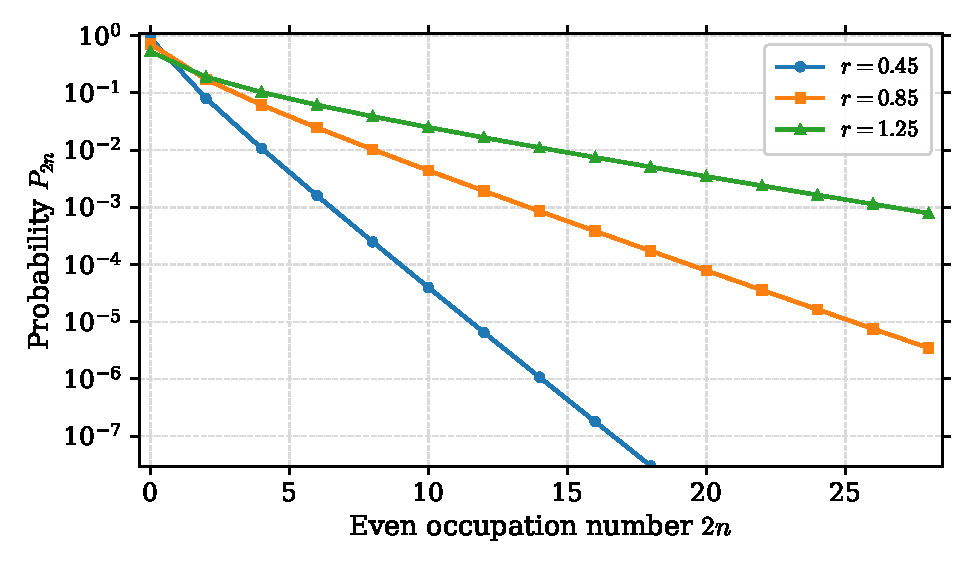
\includegraphics[width=.76\linewidth]{content/AdvancedPhysics/figures/geometry-highspin/squeezed_even_statistics.pdf}
\caption{单模压缩真空的偶数粒子数分布。概率由 \cref{eq:phys-ghs-squeezed-even-distribution} 确定，所有奇数数态的概率严格为零。}
\label{fig:phys-ghs-squeezed-even}
\end{figure}

\cref{fig:phys-ghs-squeezed-even} 中增大的压缩参数拓宽了数态分布。正交分量的噪声降低和粒子数涨落增强，描述的是同一个量子态的不同可观测量。

\begin{example}[频率突变后的激发能与粒子数]
\label{ex:phys-ghs-frequency-quench}
取固定的质量参数 $M$ 和物理正则变量 $q,p$。频率从 $\omega_0>0$ 在时间 $\tau_q$ 内改变为 $\omega_1>0$，若 $\tau_q\omega_0,\tau_q\omega_1\ll1$，可在突变近似中保持 $q,p$ 及波函数连续。两套无量纲正交分量依赖频率，不能把它们同时当成连续不变的量。

设调制前处于旧基态，求新粒子数、相对于新基态的激发能及新数态中的概率结构。

\textbf{解。} 定义 $a_\nu=\sqrt{M\omega_\nu/(2\hbar)}q+\ii p/\sqrt{2M\hbar\omega_\nu}$，$\nu=0,1$。将 $q=\sqrt{\hbar/(2M\omega_0)}(a_0+a_0^\dagger)$ 和 $p=-\ii\sqrt{M\hbar\omega_0/2}(a_0-a_0^\dagger)$ 代回，得到
\begin{align*}
a_1&=u a_0+v a_0^\dagger,\\
u&=\frac12\left(\sqrt{\frac{\omega_1}{\omega_0}}+\sqrt{\frac{\omega_0}{\omega_1}}\right),\quad
v=\frac12\left(\sqrt{\frac{\omega_1}{\omega_0}}-\sqrt{\frac{\omega_0}{\omega_1}}\right).
\end{align*}
故 $u^2-v^2=1$。若用有符号实数 $s=(1/2)\log(\omega_1/\omega_0)$，则 $u=\cosh s$、$v=\sinh s$；用非负压缩强度时取 $r=|s|$，符号由压缩相位吸收。

旧真空满足 $a_0|0_0\rangle=0$，所以
\begin{equation}
\langle N_1\rangle=\langle0_0|a_1^\dagger a_1|0_0\rangle
=v^2=\frac{(\omega_1-\omega_0)^2}{4\omega_0\omega_1}.
\label{eq:phys-ghs-quench-number}
\end{equation}
新哈密顿量的期望与新基态能量之差为
\[
\langle H_1\rangle-\frac{\hbar\omega_1}{2}
=\hbar\omega_1v^2
=\frac{\hbar(\omega_1-\omega_0)^2}{4\omega_0}.
\]
直接用旧真空的 $\langle q^2\rangle=\hbar/(2M\omega_0)$、$\langle p^2\rangle=M\hbar\omega_0/2$，也得 $\langle H_1\rangle=(\hbar/4)(\omega_0+\omega_1^2/\omega_0)$，与上式相同。

新数态中的旧真空只含偶数激发，数分布由 \cref{eq:phys-ghs-squeezed-even-distribution} 在 $r=|s|$ 处给出。调制装置对振子做功，故这里的激发不违反能量守恒。慢变化则需另用绝热条件和瞬时本征态演化，不能把突变式延用到任意调制时间。
\end{example}

\begin{figure}[htbp]
\centering
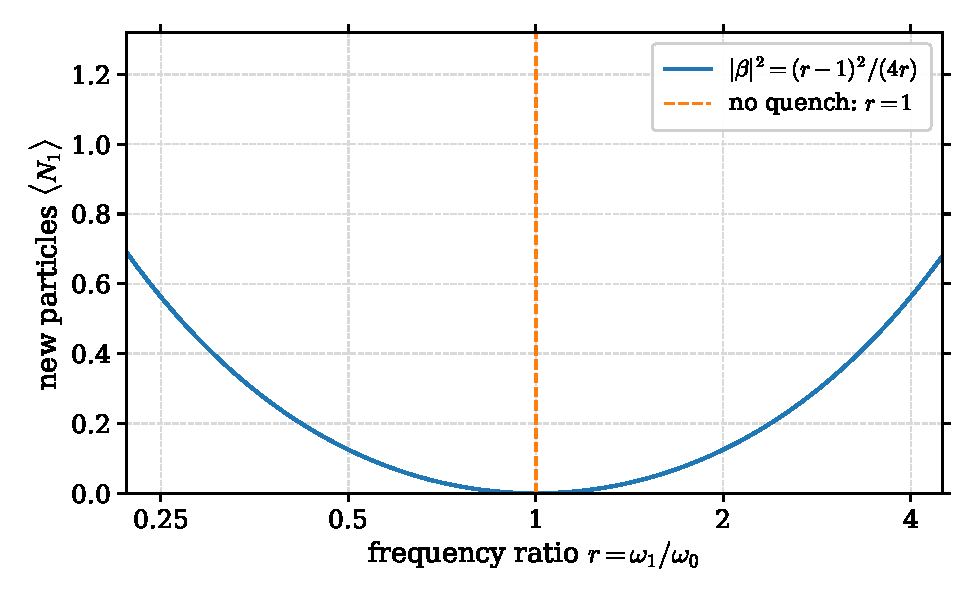
\includegraphics[width=.76\linewidth]{content/AdvancedPhysics/figures/geometry-highspin/quench_particles.pdf}
\caption{频率突变后旧真空中的新粒子数。横轴为频率比 $\omega_1/\omega_0$ 的对数刻度，曲线体现 \cref{eq:phys-ghs-quench-number} 在频率比取倒数时的不变性。}
\label{fig:phys-ghs-frequency-quench}
\end{figure}

\subsection{无限模态的压缩与高频尾}
\label{sec:phys-ghs-infinite-mode-squeezing}

\cref{fig:phys-ghs-frequency-quench} 描述一个模态。对许多模态，正则对易关系仍逐模成立，但它不足以保证两种真空都属于同一 Fock 空间。高频混合必须快到足以补偿模态数的增长。

\begin{proposition}[对角压缩真空的范数极限]
\label{prop:phys-ghs-diagonal-vacuum-limit}
取独立玻色模态 $[a_j,a_k^\dagger]=\delta_{jk}$，$b_j=a_j\cosh r_j+a_j^\dagger\sinh r_j$，$r_j\ge0$。在原真空 Fock 空间中，仅将前 $N$ 个模态改为归一化 $b_j$ 真空，记为 $|\Omega^{(N)}\rangle$。这一态列有范数极限，当且仅当
\begin{equation}
\sum_j|\beta_j|^2<\infty,\qquad\beta_j=\sinh r_j.
\label{eq:phys-ghs-diagonal-square-sum}
\end{equation}
\end{proposition}
\begin{proof}
单模递推已给出 $\langle0_j|\Omega_j\rangle=(\cosh r_j)^{-1/2}=(1+|\beta_j|^2)^{-1/4}$，相位取正。若 $N>M$，模态独立性给
\[
\langle\Omega^{(M)}|\Omega^{(N)}\rangle
=\prod_{j=M+1}^N(1+|\beta_j|^2)^{-1/4},
\]
于是
\[
\|\Omega^{(N)}-\Omega^{(M)}\|^2
=2\left[1-\exp\left(-\frac14\sum_{j=M+1}^N\log(1+|\beta_j|^2)\right)\right].
\]
该列为 Cauchy 列恰当且仅当对数级数收敛。若平方和收敛，利用 $\log(1+t)\le t$ 即得对数级数收敛；反之对数级数收敛使 $|\beta_j|^2\to0$，最终 $|\beta_j|^2\le1$，在这个尾部有 $\log(1+t)\ge t/2$，从而平方和也收敛。原 Fock 空间的完整性给出结论。
\end{proof}

\begin{example}[模态简并度参与收敛判据]
考虑幂律衰减的 Bogoliubov 混合系数，分别取非简并序列及具有幂律壳简并度的模态族。求平方和收敛对衰减指数的要求，并检查临界指数。

\textbf{解。} 若非简并模态满足 $|\beta_j|\sim Cj^{-p}$，上述判据为 $p>1/2$。若频率壳的简并度为 $g_n\sim C_1n^{q-1}$，每个模态的混合为 $|\beta_n|\sim C_2n^{-p}$，则需
\[
\sum_n g_n|\beta_n|^2\sim C_1C_2^2\sum_n n^{q-1-2p}<\infty,
\qquad 2p>q.
\]
临界 $2p=q$ 为调和级数发散。故逐模混合趋零仍不能保证无限模态真空存在于原表示中。
\end{example}

\begin{figure}[htbp]
\centering
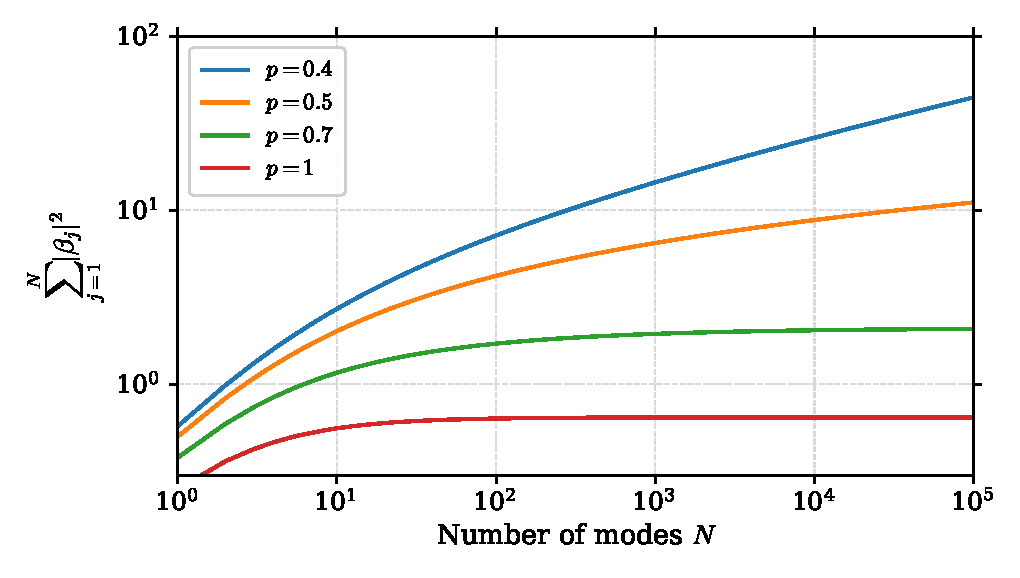
\includegraphics[width=.78\linewidth]{content/AdvancedPhysics/figures/geometry-highspin/fock_implementability.pdf}
\caption{对角混合 $|\beta_j|=(j+1)^{-p}$ 的平方和截断。$p>1/2$ 收敛，$p=1/2$ 对数增长，$p<1/2$ 幂律增长；这些是离散模态的精确求和。}
\label{fig:phys-ghs-fock-tail}
\end{figure}

\cref{fig:phys-ghs-fock-tail} 的尾部决定真空态列是否收敛。一般非对角变换 $b_i=\sum_j(\alpha_{ij}a_j+\beta_{ij}a_j^\dagger)$ 的酉实现条件是 $\beta$ 为 Hilbert--Schmidt 算子，还须满足 $\alpha\alpha^\dagger-\beta\beta^\dagger=I$ 和 $\alpha\beta^{\mathsf T}=\beta\alpha^{\mathsf T}$。这一无限维表示定理及曲空间正频的构造见《自由电子量子光学》的几何量子态章；前面的乘积证明只建立了对角真空的范数判据。
